\documentclass[a4paper]{article} % you can use the same options as for article class

%%%%%%%%%%%%%%%%%%%%%%%%%%%%%%%%%%%%%% Meta Information %%%%%%%%%%%%%%%%%%%%%%%%%%%%%%%%%%%%%%

\def\muni{Masaryk University}
\def\uvt{Institute of Computer Science}
\def\street{Botanick\'{a} 68a}
\def\psc{602\,00 Brno}

\def\projectname{AIDA Framework}

\def\reportauthor{Martin Hus\'{a}k, Jaroslav Ka\v{s}ar, Milan \v{Z}iaran}
\def\reporttitle{User Manual \& Documentation}

%%%%%%%%%%%%%%%%%%%%%%%%%%%%%%%%%%%%%% Included Packages %%%%%%%%%%%%%%%%%%%%%%%%%%%%%%%%%%%%%%

\usepackage[paper=a4paper,top=2.5cm,bottom=2.5cm,left=2.5cm,right=2.5cm,bottom=2.5cm,foot=1cm]{geometry}
\usepackage{cmap}       % cut and past support for iso-8859-2 characters
\usepackage[utf8]{inputenc}
\usepackage[default,osfigures,scale=0.5]{opensans}
\usepackage[T1]{fontenc}
\usepackage[hyphens]{url}
\usepackage{hyperref}
\usepackage[usenames, dvipsnames]{xcolor}
% \usepackage{lastpage}
\usepackage{indentfirst}
\usepackage{graphicx}
% \usepackage{booktabs}
% \usepackage{multirow}
\DeclareGraphicsExtensions{.pdf, .ps, .eps, .png}

%%%%%%%%%%%%%%%%%%%%%%%%%%%%%%%%%%%%%% Colors %%%%%%%%%%%%%%%%%%%%%%%%%%%%%%%%%%%%%%

\definecolor{projectcolor}{RGB}{93,118,168}
\definecolor{uvtcolor}{RGB}{188,4,78}
\definecolor{textcolor}{RGB}{90,90,90}
\definecolor{notecolor}{RGB}{150, 150, 150}
\definecolor{emphcolor}{RGB}{93,118,168}

%%%%%%%%%%%%%%%%%%%%%%%%%%%%%%%%%%%%%% Settings for pdf output %%%%%%%%%%%%%%%%%%%%%%%%%%%%%%%%%%%%%%

\hypersetup{%
pdftitle   = {\reporttitle},
pdfauthor  = {\reportauthor},
pdfsubject = {\projectname},
pdfkeywords= {},
%
unicode=true,                % czech in bookmarks
bookmarks=true,              % turn on creation of bookmarks
bookmarksopen=false,         % expand subsections in bookmark tab
bookmarksnumbered = true,    % chapter numbers in bookmarks
bookmarksopenlevel = 5,
%
pdfpagemode=UseOutlines,     % UseThumbs, UseOutlines (turn on bookmarks), FullScreen, None
pdfpagelayout=SinglePage,    % SinglePage, OneColumn, TwoColumnLeft, TwoColumnRight
pdfstartview=FitV,           % Fit, FitB, FitH, FitV
%
backref = false,
linkcolor = textcolor,
citecolor = textcolor,
urlcolor = textcolor,
colorlinks = true,           % on/off link boxes
hyperindex=true,
plainpages=false,            % fix duplicated pages when roman/arabic numbering is used
%
}

%%%%%%%%%%%%%%%%%%%%%%%%%%%%%%%%%%%%%% Document formating %%%%%%%%%%%%%%%%%%%%%%%%%%%%%%%%%%%%%%

\renewcommand{\sfdefault}{opensans}
\renewcommand{\familydefault}{\sfdefault}
\renewcommand{\normalsize}{\fontsize{12}{15}\selectfont\color{textcolor}}

\tolerance 9999 % big white space tolerance for better typesetting and text hyphenation

\def\verbatim@font{\color{textcolor}} % color of verbatim text

\makeatletter       % section title formating
\renewcommand\section{\@startsection {section}{1}{\z@}%
                   {-3.5ex \@plus -1ex \@minus -.2ex}%
                   {2.3ex \@plus.2ex}%
                   {\normalfont\sffamily\Large\bfseries\color{projectcolor}}}
\renewcommand\subsection{\@startsection{subsection}{2}{\z@}%
                   {-3.25ex\@plus -1ex \@minus -.2ex}%
                   {1.5ex \@plus .2ex}%
                   {\normalfont\sffamily\large\bfseries\color{projectcolor}}}
\renewcommand\subsubsection{\@startsection{subsubsection}{3}{\z@}%
                   {-3.25ex\@plus -1ex \@minus -.2ex}%
                   {1.5ex \@plus .2ex}%
                   {\normalfont\normalsize\sffamily\bfseries\color{projectcolor}}}
\makeatother

\newenvironment{itemize*}%
{\begin{itemize}%
    \setlength{\itemsep}{0pt}%
    \setlength{\parskip}{0pt}%
}{\end{itemize}}

\usepackage[pages=some,scale=1,angle=0,opacity=1]{background}
\newcommand\BackImage[2][scale=1]{%
\BgThispage
\backgroundsetup{
  contents={\includegraphics[#1]{#2}}
  }
}
\usepackage[absolute,overlay]{textpos}

% fancy verbatim and listings
\usepackage{fancyvrb}
\usepackage{listings}
\definecolor{listingbg}{RGB}{242,242,242}
\lstset{
	basicstyle=\footnotesize\ttfamily,
	captionpos=b,
	backgroundcolor=\color{listingbg},
	framesep=4pt,
	frame=single,
	breaklines=true,
	rulecolor=\color{listingbg},
	aboveskip=10pt
}

\begin{document}

% title page
{
\BackImage[width=1.4\textwidth]{fig/titlepage_bg}
\pdfbookmark[1]{Title page}{pdf_first_page}

\vspace*{5cm}

\color{white}
  \begin{center}
  \vspace{2cm} {\Huge \projectname}

  \vspace{1cm} {\huge\bfseries\MakeUppercase{\reporttitle}}
  \end{center}

  \begin{textblock}{3}(1,10)
      \hyphenpenalty=10000 % prevent names from hyphenating
         \begin{tabular}{rl }
            Authors & \reportauthor \\
             & \\
            Contact address & \muni \\
             & \uvt \\
             & \street \\
             & \psc \\
          \end{tabular}
      \hyphenpenalty=0
  \end{textblock}
  \cleardoublepage
}

\normalfont

% content page

\pdfbookmark[1]{Content}{pdf_contents}

\setcounter{tocdepth}{2}

\tableofcontents

\vspace*{\fill}

\normalfont

\pdfbookmark[1]{Acknowledgement}{Acknowledgement}
\section*{Acknowledgment}

The authors of the AIDA framework are Martin Hus\'{a}k, Jaroslav Ka\v{s}ar, Milan \v{Z}iaran. The authors would like to thank Michal Pav\'{u}k, V\'{i}t Rus\v{n}\'{a}k, and Jakub Kolman for the dashboard, and Petr Velan and Samuel \v{S}u\v{l}an for testing the framework.

% AIDA Framework integrates SPMF library\footnote{\url{http://www.philippe-fournier-viger.com/spmf/}} distributed under GPL v3 license.

There is a design paper describing the AIDA framework, see:
\begin{lstlisting}[]
Martin Husák and Jaroslav Kašpar. 2019. AIDA Framework: Real-Time Correlation and Prediction of Intrusion Detection Alerts. In Proceedings of the 14th International Conference on Availability, Reliability and Security (ARES '19). ACM, New York, NY, USA, Article 81, 8 pages. DOI: https://doi.org/10.1145/3339252.3340513
\end{lstlisting}

To cite the paper, we recommend using the following bibtex entry:
\begin{lstlisting}[]
@inproceedings{AIDAframework,
 author = {Hus\'{a}k, Martin and Ka\v{s}par, Jaroslav},
 title = {AIDA Framework: Real-Time Correlation and Prediction of Intrusion Detection Alerts},
 booktitle = {Proceedings of the 14th International Conference on Availability, Reliability and Security},
 series = {ARES '19},
 year = {2019},
 isbn = {978-1-4503-7164-3},
 location = {Canterbury, CA, United Kingdom},
 pages = {81:1--81:8},
 doi = {10.1145/3339252.3340513},
 publisher = {ACM},
 address = {New York, NY, USA},
 keywords = {alert correlation, data mining, information sharing, intrusion detection, prediction}
}
\end{lstlisting}

The development of the framework and related research were supported by the Security Research Programme of the Czech Republic 2015 - 2020 (BV III / 1 VS) granted by the Ministry of the Interior of the Czech Republic under No. VI20162019029 The Sharing and analysis of security events in the Czech Republic. 
Further research was supported by ERDF ``CyberSecurity, CyberCrime and Critical Information Infrastructures Center of Excellence'' (No.CZ.02.1.01/0.0/0.0/16\_019/0000822).

\cleardoublepage

\section{Introduction}

AIDA is an analytical framework for processing intrusion detection alerts with a focus on alert correlation and predictive analytics. The framework contains components that filter, aggregate, and correlate the alerts, and predict future security events using the predictive rules distilled from historical records. The components are based on stream processing and use selected features of data mining (namely sequential rule mining) and complex event processing. The framework was designed to be deployed as an analytical component of an alert processing platform. Alternatively, it can be deployed locally for experimentations over datasets.

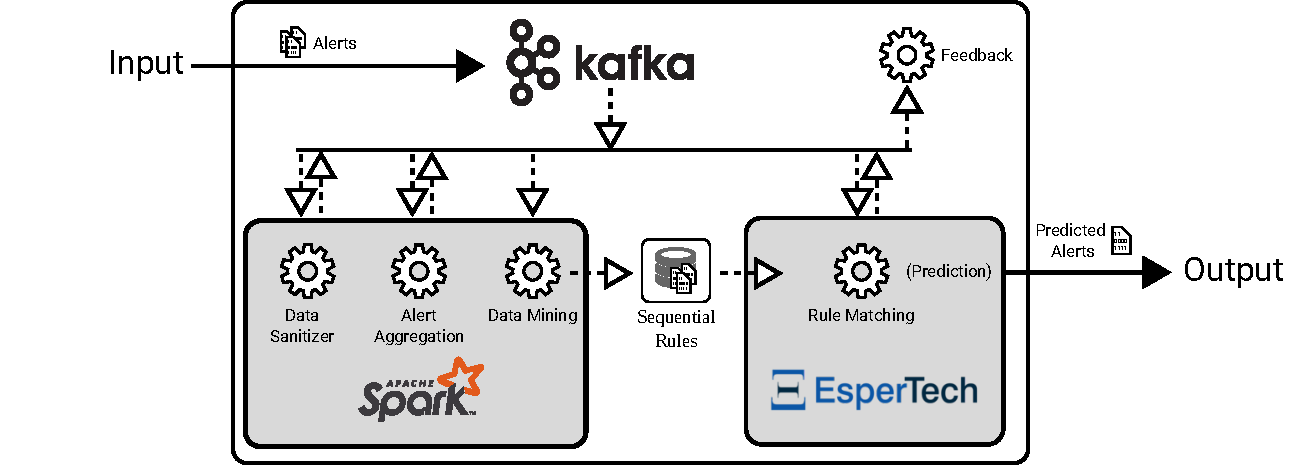
\includegraphics[width=\textwidth]{fig/aida_schema}

IDEA\footnote{\url{https://idea.cesnet.cz/}}

\begin{lstlisting}[]
OrganizationA.Honeypot1_Recon.Scanning_22,
OrganizationB.IDS1_Attempt.Login_22
==>
OrganizationA.IDS1_Attempt.Login_22
#SUPP: 0.0011 #CONF: 0.6111
\end{lstlisting}

\begin{lstlisting}[]
{
  "Format": "IDEA0",
  "ID":"f62537c2-77b8-49c7-a0a2-24c4b81b20f8",
  "CorrelID": [ % IDs of preceding alerts
        "3688762d-2efa-44a8-9ea5-34a57b3ae0c7",
        "ae6d9ac6-6389-407f-9d7e-58b9692c6eaa"
      ],
  "DetectTime": "2019-03-16T12:17:21.609+00:00",
  "Category": ["Attempt.Login"],
  "Confidence": "0.6111",
  "Description": "The source IP address follows a known pattern that is expected to continue with the event described in this message.",
  "Note": "OrganizationA.Honeypot1_Recon.Scanning_22, OrganizationB.IDS1_Attempt.Login_22 ==> OrganizationA.IDS1_Attempt.Login_22",
  "Source": [{"IP4": ["10.11.12.13"]}],
  "Target": [{"Port":[22]}],
  "Node": [
    { % Node referencing the AIDA Framework
      "Name": "OrganizationX.AIDA",
      "SW": "AIDA",
      "Type": ["Correlation", "Statistical"]
    },
    { % Node derived from the rule
      "Name": "OrganizationA.IDS1"
    }
  ]
}
\end{lstlisting}

\cleardoublepage

\section{Quick Start}

For a quick start, go to the provision directory and run Vagrant:

\begin{lstlisting}[]
cd provision
\end{lstlisting}

\begin{lstlisting}[]
vagrant up
\end{lstlisting}

AIDA framework will start in few minutes. Then, send your data to the framework using the following command (you need to have netcat installed):

\begin{lstlisting}[]
nc localhost 4164 < path_to_file_with_your_data
\end{lstlisting}

If you do not have your own data, we recommend trying AIDA framework out with our dataset\footnote{\url{http://dx.doi.org/10.17632/p6tym3fghz.1}}. Download and unzip the main file in the datase (dataset.idea.zip) and use it in the command above.

TODO run data mining

TODO update rules

TODO check outputs

\cleardoublepage

\section{Installation Instructions}

deployment

\cleardoublepage

\section{User Guide}

incl. screenshots

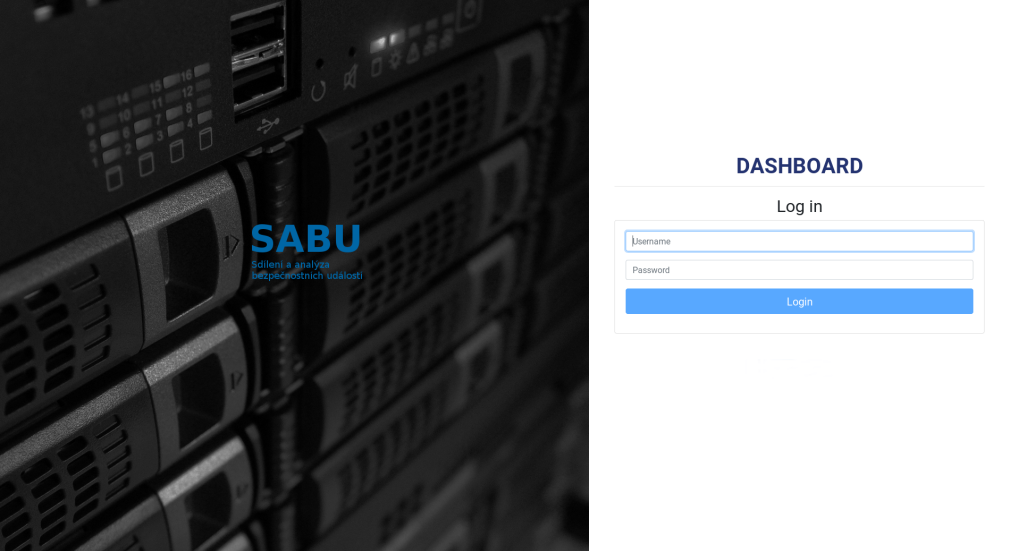
\includegraphics[width=0.75\textwidth]{fig/dashboard_login}

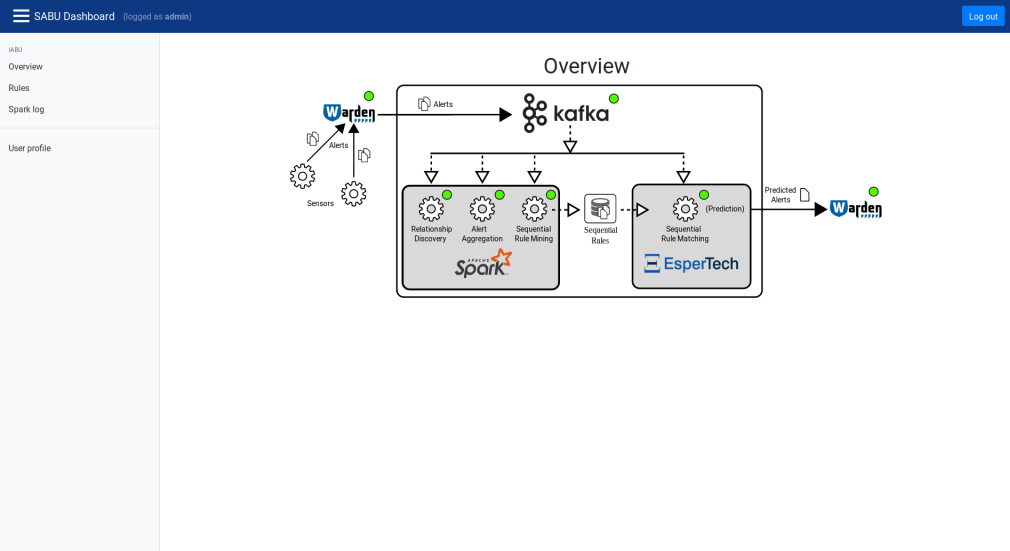
\includegraphics[width=0.75\textwidth]{fig/dashboard_overview}

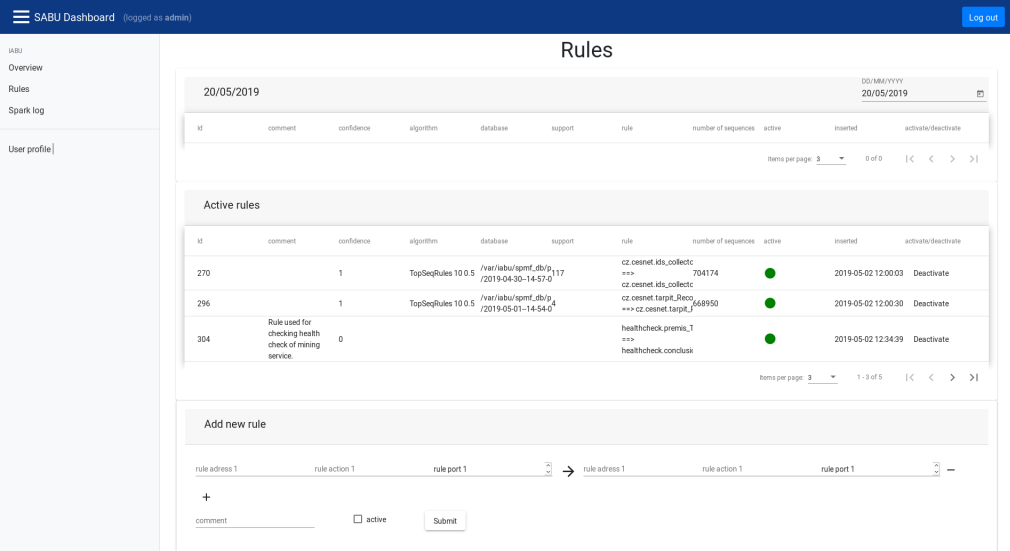
\includegraphics[width=0.75\textwidth]{fig/dashboard_rules}

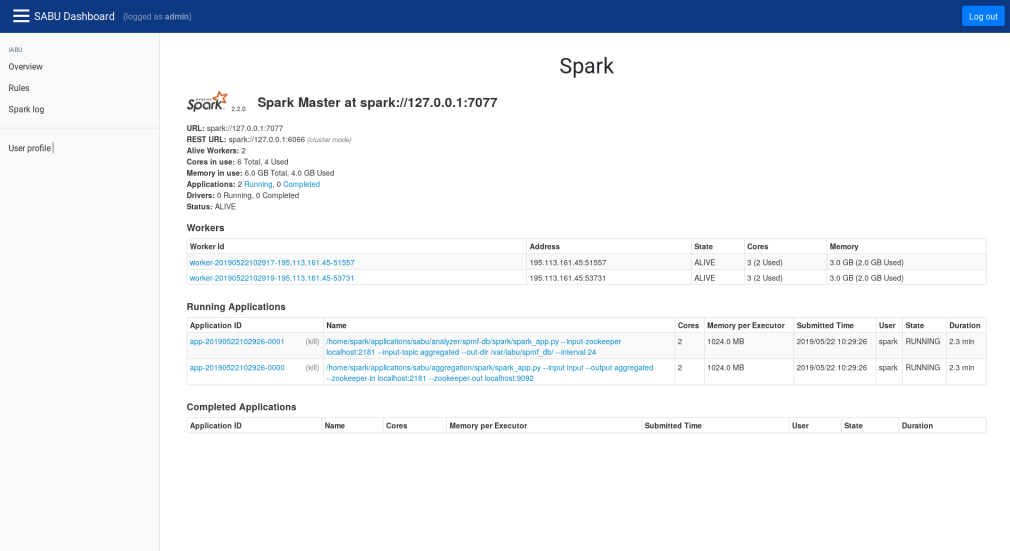
\includegraphics[width=0.75\textwidth]{fig/dashboard_spark}

\cleardoublepage

\section{Technical Documentation}

TODO

\end{document}
